\documentclass{sig-alternate-05-2015}
\usepackage{amsmath, amssymb}
% for some reason the sig document class doesn't work well with amsthm \usepackage{amsthm} 
\usepackage{thm}
\usepackage{tikz}
\usetikzlibrary{matrix}
\usepackage[all]{xy}
\usepackage{url}

\title{A graphical approach to measuring smart cities}
\author{Joshua Z. Tan, Abhishek Dubey, and Sokwoo Rhee}
\date{\today}

\theoremstyle{plain}
\newtheorem{thm}{Theorem}[section]
\newtheorem{prop}[thm]{Proposition}
\newtheorem{cor}[thm]{Corollary}
\newtheorem{lem}[thm]{Lemma}

\theoremstyle{plain}
\newtheorem{define}{Definition}
\newtheorem{example}{Example}

\theoremstyle{remark}
\newtheorem{remark}{Remark}

% editing definitions
\newcommand{\grayout}[1]{{\color{gray}#1}}
\newcommand{\redout}[1]{{\color{red}#1}}
\newcommand{\marginnote}[1]{\marginpar{\footnotesize \color{blue}#1}}

% category theory definitions
\DeclareMathOperator{\id}{id}
\DeclareMathOperator{\dom}{dom}
\DeclareMathOperator{\cod}{cod}
\DeclareMathOperator{\dvert}{Vert}
\DeclareMathOperator{\Lax}{Lax}
\DeclareMathOperator{\Hom}{Hom}
\DeclareMathOperator{\Mor}{Mor}
\DeclareMathOperator{\Ob}{Ob}
\DeclareMathOperator{\MOb}{\lvert\mspace{2mu}\cdot\mspace{2mu}\rvert}
\DeclareMathOperator{\Tr}{Tr}
\DeclareMathOperator*{\colim}{colim\;}
\DeclareMathOperator{\Coll}{Col}
\def\op{^{\text{op}}}
\def\dom{\tn{dom}}
\def\cod{\tn{cod}}

\newcommand{\Cat}[1]{\mathsf{#1}}
\def\Set{\Cat{Set}}
\def\Poset{\Cat{Poset}}
\def\Bool{\Cat{Bool}}
% end category theory definitions

% begin additional definitions
\def\Ind{\Cat{Ind}}
\def\Bayes{\Cat{Bayes}}
\def\Rand{\Cat{Rand}}
\def\Cor{\textnormal{Cor}}
% end additional defintions

\begin{document}
\maketitle

% Intuition: how the effects correlate serves as a proxy for a "holistic" vision of the intended effect.

% Event structures? A valuation functor over consistent subsets that respects the consistency condition. But how do you assign a correlation-like value to arbitrary indicators, then respects the idea that the correlation between two indicators is just the correlation?

\redout{Suggestions from Ed: make sure to motivate the math before even mentioning ``hybrid indicator frameworks'' as a solution. There are things called ``process indicators'' in systems engineering, which are a bit different from KPIs. We need a completeness theorem stating that the diagrammatic calculus for indicator frameworks actually models all possible indicator frameworks and correlations.}

\redout{Publication strategy: use this paper to focus on formalizing just indicator frameworks\emph{without mentioning the hybrid part}, with a diagrammatic calculus, and publish in the CPS week workshop. Create an application-focused paper, again without the `hybrid' part, that connects this workshop paper with the CPS Framework, and publish that in Ed's special issue. Finally, develop in late spring a full hybrid indicator framework paper.}


\section{Introduction}
Suppose we take as our starting point a simple diagram of correlations between the system variables of a complex system, as below.

\begin{figure}[h!]
\includegraphics[width=\linewidth]{portland}
\end{figure}

The diagram correlates the measurement variables of an air pollution monitoring system with other, partially-observable variables like traffic composition, mechanical turbulence, the presence of sunlight. It presents an intuitive---and apparently useful---description of a system at large. We would like to clarify the meaning of this diagram, and of others like it, by giving the diagram a precise mathematical semantics. Clarifying the meaning of the diagram will not only make it more useful; it will allow us to connect this simple, non-causal picture of the system with more sophisticated \emph{causal} models.

In this essay, we develop a diagrammatic calculus for correlations between random variables. Broadly, we expect our diagrammatic calculus to have a notion of \emph{process} (i.e. correlations), \emph{state} (i.e. random variables), and \emph{effect} (i.e. random variables). 
\begin{figure}[h!]
\centering
\includegraphics{process}
\end{figure}
These are needed to capture the operations of composing correlations in sequence, called \emph{composition}, and combining them in parallel, called \emph{tensoring}. Composition and tensoring are to be represented, respectively, as below:
\begin{figure}[h!]
\centering
\includegraphics{composition}
\end{figure}

The semantics of such diagrams are governed by the theory of monoidal categories, which is surveyed in \cite{selinger09}.

There are three reasons for our focus on correlations. First, our choice is motivated by practical considerations in the use of (key performance) indicator frameworks, especially as they are used in city planning and project governance. Such indicator frameworks present `relevant' system variables to a human decision-maker, but the determination of `relevant' becomes difficult as the system increases in size and complexity. Since indicator frameworks are so structurally simple, one of the few structures we can define on them is correlation. Second, correlations are practical; in many settings involving multivariate data, correlations are the analyst's workhorse. In observational studies of complex systems, often the best we can do is derive correlations, since observational data ``from nature'' rarely support conditional relations of the sort sought in laboratory experiments. Finally, part of the aim of this paper is to clearly distinguish causal from non-causal models, and correlations seem like a core feature of any non-causal model of multivariate data. % All other tools, from conditional probability to dynamical systems to 

% In many of our approaches to complex systems modeling, we have taken for granted an underlying causal model of the world.

% Some causal models are embedded in our mathematical assumptions, like in the conditional dependence of variables, and others are explicit, such as in process theories of measurement.

NB: Correlations are rarely composed in practice because we can usually compute the composite correlation directly from the data. If we lack the data, then we can almost always do some estimation of parameters and then use the learned model (e.g. a Kalman filter or dynamical Bayes network) to estimate the correlation. However, the use of the learned model typically incurs a causal framework. % When we use measurements, we are not invoking the underlying probabilities. Selling point: don't have to look at big collections of data. So all the different performance measures, we want to map them into a single grade e.g. 0-100. So to turn it into a single value or indicator.

% CHECK: does the correlation actually define a metric?

% Future work: we can also turn this into a supervised learning problem. We learn the correlations, present it to an expert, and ask is it right? Then the expert can sort groups into good and bad groups.

\section{Background}
Even within the constraints of a process theory, there are still a number of diagrammatic approaches to correlation and covariance. In this section, we will go over three examples: the traditional Hilbert space interpretation of random variables, the Bayesian approach of Coecke and Spekkens \cite{coecke_spekkens}, and graphical models such as those surveyed in \cite{lauritzen96}. % One, which we denote $\Rand$, defines the correlation as an inner product; another by \cite{coecke_spekkens}, which we call $\Bayes$, describes (perfect) correlation as a certain condition on a joint state.

The most straightforward approach, which we call $\Rand$, uses the fact that real-valued, standard random variables over some fixed probability space $(\Omega, \mathcal{F}, \mathbb{P}$) form an (infinite-dimensional) Hilbert space $\mathcal{H}$ where the inner product $\langle X, Y \rangle$ is just the covariance/correlation $\mathbb{E}(XY)$. The objects of the category $\Rand$ are subspaces $H$ of $\mathcal{H}$, morphisms are unitary matrices of the appropriate dimensions, composition $g \circ f : H \to H'$ is given by matrix multiplication, and the tensor is the matrix tensor product with unit $\mathbb{R}$. A state of $H$ is a normalized vector representing a specific random variable (qua probability distribution) in the subspace $H$.

With this setup, the correlation between two standard random variables is just the inner product in $(\Omega, \mathcal{F}, \mathbb{P})$, i.e. \[\langle X, Y \rangle := \mathbb{E}(XY) / (\sigma_X \sigma_Y) = \mathbb{E}(XY).\] It is depicted:
\begin{figure}[h!]
\centering
\includegraphics{innerproduct}
\end{figure}

\cite{coecke_spekkens} gives a similar graphical calculus for Bayesian inference. Restricting to standard probability, objects of the category $\Bayes$ are natural numbers, morphisms from $m$ to $n$ are $n \times m$ stochastic matrices, composition is matrix product, and the monoidal product is the matrix tensor product. Normalized states are probability distributions over the set ${1, ..., n}$:

\begin{figure}[h!]
\centering
\label{bob_normalized_state}
\includegraphics[width=\linewidth]{bob_normalized_state}
\end{figure}

A joint state is a normalized state over the composite object ${1, ..., mn}$. A joint state is uncorrelated when it can be decomposed into a tensor product, and perfectly correlated when it can be represented as a delta function. In $\Bayes$, uncorrelated and perfectly correlated joint states are depicted, respectively:

\begin{figure}[h!]
\centering
\label{bob_uncorrelated_state}
\includegraphics[width=\linewidth]{bob_uncorrelated_state}
\end{figure}

\begin{figure}[h!]
\centering
\label{bob_correlated_state}
\includegraphics[width=\linewidth]{bob_correlated_state}
\end{figure}

The work of \cite{coecke_spekkens} is itself related to older work on the categorical foundations of probability initiated by Lawvere in \cite{lawvere62}. In that paper, the category of probabilistic mappings has objects Borel spaces $(X, \Sigma_X)$ and morphisms Markov kernels; a Markov kernel $T : (X, \Sigma_X) \to (Y, \Sigma_Y)$ represents a function $T : \sigma_Y \times X \to [0,1]$ that assigns to each $x \in X$ and each measurable set $B \in B_Y$ the probability of $B$ given $x$, denoted $T(B | x)$; in this way, each random variable can be represented as a morphism between Borel spaces (technically, the probability measure of $T$), and the composition of random variables corresponds to marginalization. % A random variable is a... 

\redout{Finally, in Bayesian statistics and machine learning, a variety of more generic graphical approaches, called graphical models, have been developed to model the conditional (in)dependence of multivariate random variables; the joint distribution over all the random variables in a graphical model is the product of their conditional distributions. The upshot is that complex questions about joint distributions of many interrelated variables can be answered in terms of the topology of the graph. 

[Need more explanation and figures.]}

$\Bayes$ and similar formalisms give a semantics for probabilistic reasoning, often with a specific causal model. Causal models are useful for interpreting the results of an experiment. It is not useful, generally speaking, when the data do not provide evidence for causation, such as in purely observational studies of complex systems. We want to carefully distinguish the causal aspects of our models from their non-causal aspects, and the first step is to develop a coherent framework for \emph{non-causal} reasoning. % more positive way of describing non-causal: what it means to have a status quo...

% \redout{A third approach fixes a specific Hilbert space of random variables and interprets it as a Lawvere metric space. But is there a monoidal product in this space? Even if not, and there is no graphical interpretation, would there still be a reason to do this?}

\section{Indicator Frameworks}
In this section, we define the category $\Ind$ of abstract indicator frameworks and give an example, with diagrams, of a concrete indicator framework.

Before giving the definition of the category $\Ind$ of abstract indicator frameworks, we will go through some of the statistical justification. Suppose that we have a correlation between random variables $X$ and $Y$ and another one between $Y$ and $Z$. What can we say about the correlation between $X$ and $Z$? One obvious guess would be 
\begin{equation}\label{eqn:guess1}\Cor(X,Y) = \Cor(X,Y)\Cor(Y,Z).\end{equation}
Of course we know that (\ref{eqn:guess1}) is, in general, false. But it is, under certain conditions, still the best guess. The following result is an exercise in \cite{statistics_textbook}.

\begin{lem}If $a = \Cor(X,Y)$ and $b = \Cor(Y,Z)$, then 
\begin{gather}
\Cor(X,Z) \geq ab - \sqrt{1-a^2}\sqrt{1-b^2} \\ 
\Cor(X,Z) \rangle \leq ab + \sqrt{1-a^2}\sqrt{1-b^2}
\end{gather}
\end{lem}

\begin{proof}
WLOG, assume that $A,B,C$ are standard variables with zero mean and unit variance, since the correlation is invariant under changes to mean and variance. We can write $X = a Y + O_Y^X$ and $Z = b Y + O_Y^Z$ where, by assumption, $O_Y^X, O_Y^Z$ are random variables uncorrelated with $Y$.

Then $\langle X, Z \rangle = \Cor(X,Z) = \langle aY + O_Y^X, bY + O_Y^Z \rangle = ab + \langle O_Y^X, O_Y^Z \rangle$.

We can use the Cauchy-Schwarz inequality to bound $\langle O_Y^X, O_Y^Z \rangle$ from above and from below, giving the lemma.
\end{proof}

The lemma tells us that there is a range of possible values, centered around $\Cor(X,Y)\Cor(Y,Z)$, for the composite correlation. % We can interpret the size of this range as a ``likelihood score'' on (\ref{eqn:guess1}); in the case where $\Cor(X,Y) = \Cor(Y,Z) = 1$, the range is $[ab,ab]$ and (\ref{eqn:guess1}) is 100\% likely to be true; in the cases where one correlation is $-1$ and the other is 1, or when both are 0, the range is $[-1,1]$ and (\ref{eqn:guess1}) is least likely to be true.
In such a situation, we may ask what is the obstruction, given $\Cor(X,Y)$ and $\Cor(Y,Z)$, to knowing the canonical or `true' correlation of their composite. Reading the proof of the lemma, we know this is just the correlation $\langle O_Y^X, O_Y^Z \rangle$. Intuitively, since $\langle O_Y^X, Y \rangle = \langle O_Y^Z, Y \rangle = 0$, they give `all' the extra information relevant to $\Cor(X,Z)$. % One imagines $\langle O_Y^X, O_Y^Z \rangle$ as an old balancing scale with one variable on either side; the fact that the scale is fair corresponds with the fact that neither $O_Y^X$ nor $O_Y^Z$ have any correlation with $Y$.

Now, another way of telling the same story above is to say that we are interested in how correlations between two variables, $X$ and $Z$, may `factor through' an intermediate variable, $Y$, in such a way that the diagram below commutes.
\begin{figure}[h!]
\centering
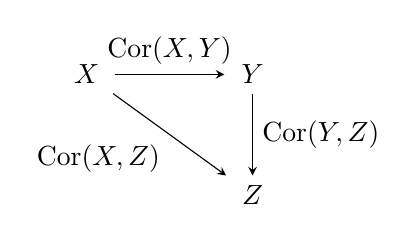
\begin{tikzpicture}
  \matrix (m) [matrix of math nodes,row sep=3em,column sep=4em,minimum width=2em]
  {
     X & Y \\
     & Z \\};
  \path[-stealth]
    (m-1-1) edge node [above] {$\Cor(X,Y)$} (m-1-2)
    (m-1-2) edge node [right] {$\Cor(Y,Z)$} (m-2-2)
    (m-1-1) edge node [below left] {$\Cor(X,Z)$} (m-2-2);
\end{tikzpicture}
\end{figure}

In this paper, we have a more specific way of thinking about this diagram: if $X$ and $Z$ are fixed, how can we design a random variable $Y$, or a set of random variables $\{Y_i\}$, such that $X$ and $Z$ are maximally correlated?

Now, suppose we had two variables, $X$ and $Z$, and we wanted to `tensor' them in a way that captures the same extra information relevant to $\Cor(X,Z)$, given any random variable $Y$ or set of random variables, possibly correlated with each other. 

I.e. so that $\Cor(X \otimes_Y Z, Y) = \langle O_Y^X, O_Y^Z \rangle$.

Perfectly-correlated variables duplicate knowledge; the more correlated two variables are, the more information is lost when they are combined.

 which is perfectly correlated with another variable, it does not add much to our knowledge of the world. perfectly correlated variables which then correlate do not offer much more information about 

Now suppose we have two correlations, $\Cor(X,Y)$ and $\Cor(U,V)$, ``parallel'' to each other in the sense.

The natural product between random variables should be a tensor product.

Suppose we had some initial notion of how ``significant'' certain random variables was, relative to other variables.


Of course, we didn't have to derive this result to guess 

Now suppose that we have multiple correlations $\Cor(X,Y_i)$ and $\Cor(Y_i,Z)$. Can we say anything more about the correlation between $X$ and $Z$?

 for which we have correlations between $X$ and $Z$.
\[ \langle X , Z \rangle = \frac{1}{n} \sum_{i \in B}^n \langle X,Y_i \rangle \langle Y_i, Z \rangle.\] 
This assumes, however, that all the correlations are equally significant in supplying the correlation. Moreover, it fails to square with our intuition

\begin{define}The category $\Ind$ of indicator frameworks takes objects as finite-dimensional Hilbert spaces, morphisms from $V^m$ to $V^n$ as an $n \times m$ matrix of correlation coefficients, and composition as the correlation matrix generated by the following equation: 

\end{define}

\begin{lem}$\Ind$ is a symmetric monoidal category with tensor $\otimes$ and monoidal unit $\mathbb{C}$.
\end{lem}

\begin{proof}
First, we can define states: a state.
\end{proof}

Given this monoidal structure, a state is a [0,1]-valued vector in that Hilbert space, which is interpreted as a ``trustworthiness'' or ``prior'' vector on each of the indicators. An effect is interpreted as a ``priority'' vector on a (typically smaller) set of indicators.

In essence, the idea is to treat indicators as something closer to \emph{features} of a given optimization problem, rather than as random variables.

% We're probably going to have to introduce some method of measuring ``failure to correlate''.

% Alternately: correlation is the projection of one random variable (imagined as a vector) onto another random variable.

% This paper is the first in a series meant to articulate \emph{hybrid indicator frameworks}. The goals of this paper are (1) to give a graphical formalism for correlation, (2) to place the choice of `relevant' system variables in the context of a process theory, and (3) to say what it means for correlations to be verified by data obtained by `measuring' the system variables, and (4) to say what it means for correlations to verify or support causal models.

% [Justify the way we have defined this category in relation to what's already out there.]

% In our hypothetical category $\Ind$, what is a joint state, what is a product state, what is an entangled state? What is an effect, is there an inner product (i.e. are there adjoints?)? What are the scalars in the monoidal category? What is discarding?

\section{Applications}
In later work, we will use $\Ind$ to give a precise definition of ``hybrid indicator frameworks'' that relate non-causal information with causal models such as those found in \cite{coecke_spekkens} or \cite{fong13}. For now, even without mentioning causal models, we can set up interesting questions from statistics and analyze them using $\Ind$.

\redout{TO DO: build an example optimization.}

% non-causal theories, causal models of the same (non-causal) data.
 
\section{Conclusion}

\section{Misc. Notes}
% \footnote{The reason for wanting a process theory of the variables represented in the correlation diagram is based on the intuition that each variable represents a functional component of a cyber-physical system, not a node in a network; this suggests a mathematical interpretation of the diagram should have more in common with the semantics of computation than with the modeling of complex networks.} 

Correlation theory wishlist
\begin{enumerate}
\item Cost heuristic on (sets of) indicators, such that imposing a state and an effect creates an optimization problem. Recall: \emph{For a given policy or project, what is the `right' set of indicators to measure it? Subtext: ``holistic''?} % Is there a duality between indicators as ``features'' in a given data analysis problem, and indicators here as something we are optimizing over---picking the best features. Akin to states vs. effects?
\item A super-indicator is a ``conceptual'' indicator, whose correlation  is not set down in terms of its data, and which is supposed to represent the priorities of the Mayor, and it should be definable, at least partly, in terms of the particular projects and policies related to it.

``Super'' indicators, e.g. quality-of-life, that represent high-level goals disconnected from reality or data, as joint indicators with special properties. A super-indicator (or any joint indicator) like quality-of-life should be at least partially defined in terms of the projects and policies which can affect it. % A person has an ``intuitive sense of what they want''. We want to view this intuitive sense as just the decomposition rule into measurable things. This follows what a city person does in practice; they want to ``improve the transportation system''.
\item Statistical significance of the correlation. E.g. how can we check that we have enough data points, or represent the fact that we don't have enough? % Also, in some situations, even if we do find a highly significant correlation, then this could be attributed not to the direct relation of the quantities but just because they are both correlated to the same confounding factor. How do we deal with this?
\item Correlation of residuals? % Any uptrending or down-trending metric will be highly-correlated. When this problem arises, try as a solution to remove the uptrend and then measure the correlation of residuals.
\item ``Knowledge about the indicators'' can be formalized through functors from other categories to $\Ind$.
\end{enumerate}

Process theory wishlist:
\begin{enumerate}
\item Measurements of state % What is a policy or project? A process. What is evaluation or measurement? It is a 0,1 (or, possibly, something in [0,1], in a quantile, or, much more generally, a value in any symmetric monoidal category).
\item Correlations between indicators
\item General processes in the underlying complex system
\end{enumerate}

Arbitrary system variables in the complex system do not have an assigned meaning of measurement (in other ways, we're not collecting data on them)... but that doesn't mean they don't matter. Similarly [but in what way?], there is no underlying reality or total state of the complex system; the state may not be measurable, but that doesn't mean it doesn't matter. We should be able to put them into larger equations that govern the whole.

% What is an indicator (or a sensor)? It's a ``measurement tool''; alternately, you can think of it as a ``feature''; something that, given an input, outputs a 0 or a 1 depending on whether or not a stated effect has occurred. In the ONB formulation, it's a test for whether the input vector is equal to the stated effect.

\bibliographystyle{abbrv}
\bibliography{paper} 

\end{document}
